\documentclass[10pt,UTF8]{book} %% ctexart

\title{\textbf{算法与数据结构}}
\author{钱锋\thanks{Email: strik0r.qf@gmail.com}${}^,$\thanks{
    西北工业大学软件学院, School of Software, Northwestern Polytechnical University, 西安 710072
}}

\usepackage{ctex}
\usepackage{graphicx}
\usepackage[toc]{multitoc}
\usepackage{booktabs}
\usepackage{longtable}
\usepackage{amsthm, amssymb, amsmath, mathrsfs, mhchem}
\usepackage{tikz,circuitikz}
\usetikzlibrary{decorations.markings, angles, quotes}
\usetikzlibrary{shapes,arrows.meta,positioning}
\usepackage{tikz-cd}
\usepackage{pgfplots}
\usepackage{tikz-3dplot}
\usepackage{extpfeil}
\usepackage{diagbox}
\usepackage{float}
\usepackage{hyperref}
\hypersetup{hidelinks,
    colorlinks = true,
    allcolors = black,
    pdfstartview = Fit,
    breaklinks = true}
\usepackage{caption}
\usepackage{enumitem}
\usepackage{siunitx}
\usepackage{subcaption}
\usepackage{tasks}

\usepackage{fancyhdr} % 用于自定义页眉页脚


% 设置页眉页脚样式
\fancypagestyle{plain}{%
    \fancyhf{} % 清空页眉页脚
    \fancyhead[RO,LE]{·\thepage·} % 页眉显示页码, RO表示奇数页右侧, LE表示偶数页左侧
    \fancyhead[LO]{\nouppercase{\rightmark}} % 页眉显示小节标题, LO表示奇数页左侧
    \fancyhead[RE]{\nouppercase{\leftmark}} % 页眉显示章节标题, RE表示偶数页右侧
    \renewcommand{\headrulewidth}{0.4pt} % 设置页眉横线的宽度
    \renewcommand{\footrulewidth}{0pt} % 取消页脚横线
}

\renewcommand{\headrule}{\hrule width\textwidth height\headrulewidth\vskip-\headrulewidth}

% % 取消奇偶页的页眉偏移
% \fancyhfoffset[RO,LE]{0pt}

% % 取消奇偶页的页眉偏移
% \fancyhfoffset[RO,LE]{0pt}

% 定义取消页眉的命令
\newcommand{\cancelheader}{%
    \fancyhead{} % 清空页眉
    \renewcommand{\headrulewidth}{0pt} % 取消页眉横线
    \renewcommand{\footrulewidth}{0pt} % 设置页脚横线的宽度
}

\renewcommand{\chaptermark}[1]{\markboth{第 \thechapter 章 \hspace{1em} #1}{}}
\renewcommand{\sectionmark}[1]{\markright{\thesection \, #1}}
\usepackage{titlesec} % 定义标题样式

% 设置 chapter 标题样式
\titleformat{\chapter}[hang]{\centering\heiti\Large\bfseries}{第\,\thechapter\,章}{1em}{}

% 定义 section 标题格式
\titleformat{\section}[hang]{\heiti\centering\large\bfseries}{\thesection}{1em}{}

% 定义 subsection 标题格式
\titleformat{\subsection}[hang]{\heiti\bfseries}{\textbf{\thesubsection}}{1em}{}

% 定义 subsubsection 标题格式
\setcounter{secnumdepth}{3}
\renewcommand\thesubsubsection{\arabic{subsubsection}.}
\titleformat{\subsubsection}[hang]{\kaishu}{\quad\quad\thesubsubsection\,\,}{0em}{}

% % 重新定义 textbf
% \let\oldtextbf\textbf
% \renewcommand{\textbf}[1]{{\heiti\oldtextbf{#1}}}

% % 在导言区重新定义 \normalsize 命令
% \makeatletter
% \renewcommand\normalsize{%
%    \@setfontsize\normalsize{10.5pt}{12pt}%
%    \abovedisplayskip 8\p@ \@plus2\p@ \@minus5\p@
%    \abovedisplayshortskip \z@ \@plus3\p@
%    \belowdisplayshortskip 6\p@ \@plus3\p@ \@minus3\p@
%    \belowdisplayskip \abovedisplayskip
%    \let\@listi\@listI}
% \makeatother



% 设置页边距和对齐
% \usepackage[
%     paperwidth=185mm,
%     paperheight=260mm,
%     top=35mm,
%     bottom=25mm,
%     left=18mm,
%     right=18mm,
%     footskip=15mm % 通过这里的值来调整页脚与正文内容的垂直距离
% ]{geometry}

\usepackage[
    paperwidth=210mm,
    paperheight=297mm,
    top=40mm,
    bottom=31.8mm,
    left=25.4mm,
    right=25.4mm,
    footskip=15mm % 通过这里的值来调整页脚与正文内容的垂直距离
]{geometry}

% \usepackage[
%     paperwidth=195mm,
%     paperheight=270mm,
%     top=40mm,
%     bottom=25mm,
%     left=23.5mm,
%     right=23.5mm,
%     footskip=15mm % 通过这里的值来调整页脚与正文内容的垂直距离
% ]{geometry}
\usepackage{mdframed}
\mdfsetup{
  linewidth=0.4pt,
  frametitlebackgroundcolor=white, % 或者 transparent
  frametitlefont=\heiti\bfseries,
  frametitleaboveskip=10pt,
  frametitlebelowskip=5pt,
  frametitlealignment=\raggedright % 新增此行
}
\usepackage{fontspec}
% 设置 Menlo 字体
\setmonofont{Menlo}
\usepackage{fancyvrb}
\usepackage{xcolor}
\usepackage{listings}

\definecolor{string}{HTML}{067D17}
\definecolor{comment}{HTML}{8C8C8C}
\definecolor{keyword}{HTML}{0033B3}
\definecolor{class_field}{HTML}{871094}

\lstset{breaklines}
%这条命令可以让LaTeX自动将长的代码行换行排版
\lstset{extendedchars=false}
%这一条命令可以解决代码跨页时,章节标题,页眉等汉字不显示的问题
\lstset{escapeinside={(*}{*)}}

\lstset{
    basicstyle=\small\ttfamily\heiti,
    numbers=left,
    numberstyle=\scriptsize\fontspec{Menlo}, % 使用 Menlo 字体
    stepnumber=1,
    numbersep=8pt,
    frame=leftline,
    xleftmargin=2em, % 调整代码块的左边界
    framexleftmargin=0pt, % 调整边框的位置
    breaklines=true,
    keywordstyle=\bfseries\color{keyword},          % keyword style
    commentstyle=\heiti\color{comment},       % comment style
    stringstyle=\color[HTML]{067D17},
    showstringspaces=false,
    % string literal style
    % escapeinside={\%*}{*)},            % if you want to add LaTeX within your code
    % morekeywords={}               % if you want to add more keywords to the set
}

\usepackage{smartdiagram} % 表格对角线
\everymath{\displaystyle}
\usepackage{tasks}

\begin{document}
\newtheoremstyle{mytheoremstyle}
    {1.5ex}                                         % Space above
    {1.5ex}                                         % Space below
    {}                                              % Font for body
    {}                                              % Indent amount
    {\bfseries}                                     % Font for head
    {}                                              % Punctuation after head
    {0.5em plus 0.2em minus 0.1em}                  % Space after head
    {\thmname{#1}\thmnumber{ #2}.\thmnote{ (#3).}}

\theoremstyle{mytheoremstyle}
\newtheorem{definition}{定义}[section]
\newtheorem{example}{例}[section]
\newtheorem{exercise}{习题}[section]
\newtheorem{code}{程序清单}[section]
\newtheorem*{result}{运行结果}

\newtheoremstyle{my2theoremstyle}
    {1.5ex}                                         % Space above
    {1.5ex}                                         % Space below
    {\kaishu}                                              % Font for body
    {}                                              % Indent amount
    {\bfseries}                                     % Font for head
    {}                                              % Punctuation after head
    {0.5em plus 0.2em minus 0.1em}                  % Space after head
    {\thmname{#1}\thmnumber{ #2}.\thmnote{ (#3).}}

\theoremstyle{my2theoremstyle}
\newtheorem{thm}{定理}[section]
\newtheorem{law}{定律}[section]
\newtheorem{educt}{推论}
\newtheorem{prop}{命题}
\newtheorem{lemma}{引理}
\newtheorem{axiom}{公理}
\newtheorem{property}{性质}

\newtheoremstyle{my4theoremstyle}
    {1.5ex}                                         % Space above
    {1.5ex}                                         % Space below
    {}                                              % Font for body
    {}                                              % Indent amount
    {\bfseries}                                     % Font for head
    {}                                              % Punctuation after head
    {0.5em plus 0.2em minus 0.1em}                  % Space after head
    {\thmname{#1}.}

\theoremstyle{my4theoremstyle} \newtheorem*{sol}{解}

\newtheoremstyle{my3theoremstyle}
    {1.5ex}                                         % Space above
    {1.5ex}                                         % Space below
    {}                                              % Font for body
    {}                                              % Indent amount
    {\kaishu}                                       % Font for head
    {}                                              % Punctuation after head
    {0.5em plus 0.2em minus 0.1em}                  % Space after head
    {\thmname{#1}\thmnumber{ #2}.\thmnote{ (#3).}}

\theoremstyle{my3theoremstyle} \newtheorem*{remark}{注}
\newtheorem*{cmt}{评注}
% 使用 IEEE 样式
\ctikzset{logic ports=ieee}

\pagestyle{empty}
\begin{titlepage}
    \thispagestyle{empty}
    \centering
        \vspace*{3cm}
        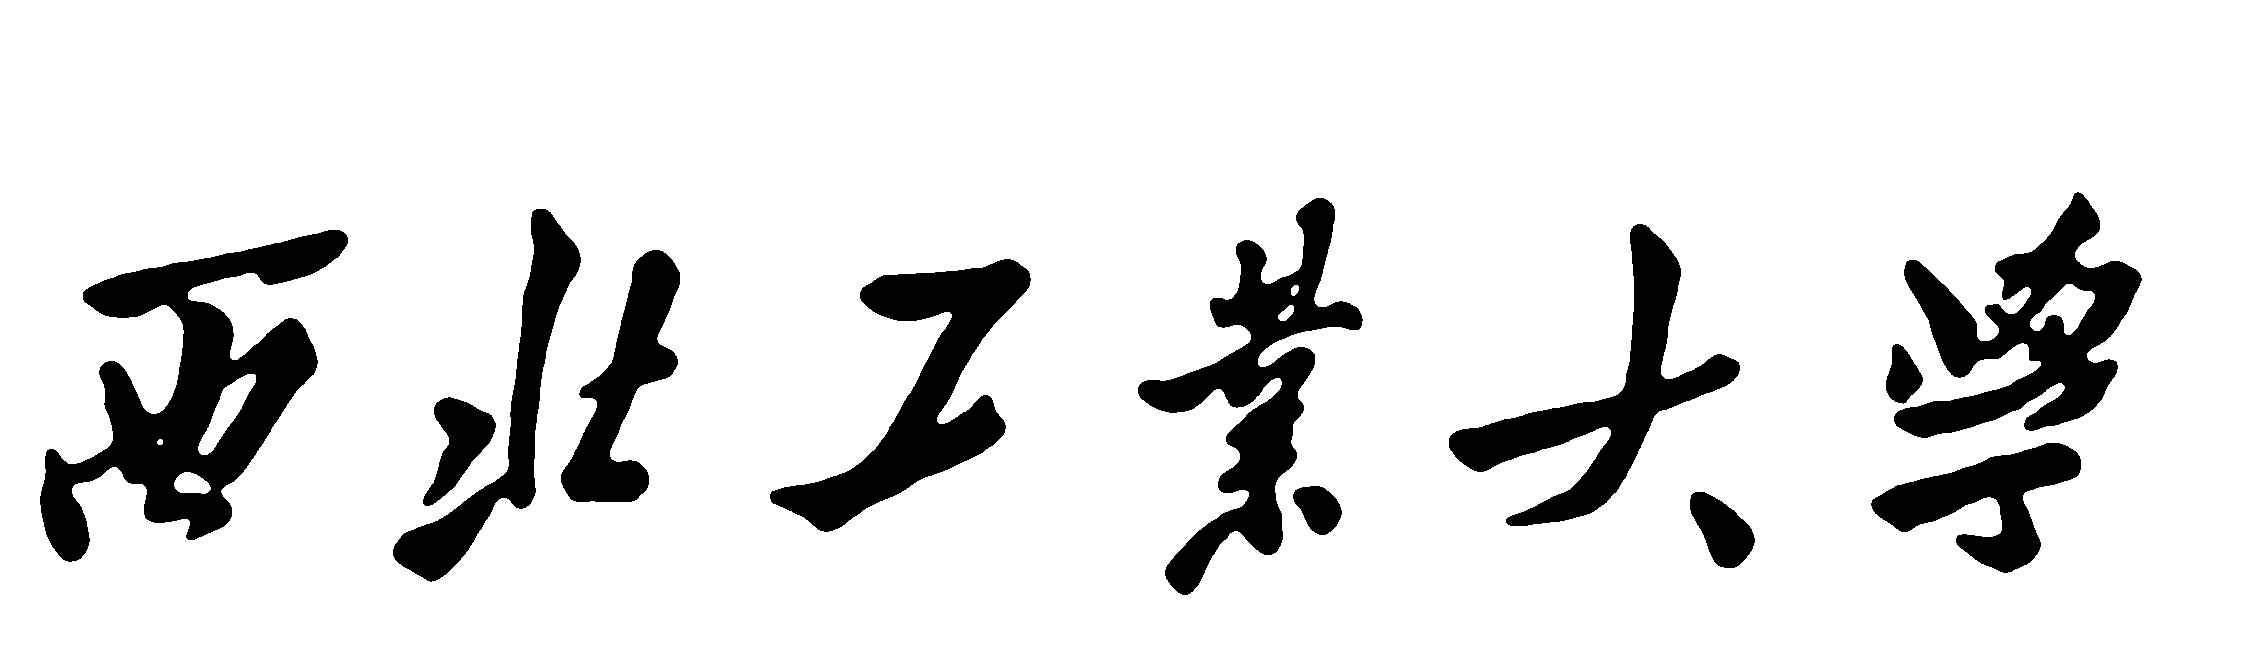
\includegraphics[width=0.5\textwidth]{pic/npu_2.png}\par
        \vspace{1em}
        
\includegraphics[width=0.5\textwidth]{pic/npu_1.png}\par
    \vspace*{1em}
        \begin{center}
            \Huge \heiti \textbf{算法与数据结构}

            Algorithms and Data Structures
        \end{center}

        \vspace{14em}
        \begin{center}
        \songti

        \kaishu 软件学院 \, \heiti\textbf{钱锋} \quad \songti 编
        \vspace{0.5em}

    \today
    \end{center}
\end{titlepage}
\cleardoublepage
\maketitle
\cleardoublepage
\frontmatter
\newpage
\pagestyle{plain}
\makeatother

\pagenumbering{roman} % 切换回罗马数字页码
\addtocontents{toc}{\protect\thispagestyle{empty}}
\pagestyle{plain}
{\tableofcontents}
\newpage
\thispagestyle{empty}
\cleardoublepage % 确保正文从奇数页开始


% 设置章节标题页的页眉和页脚为空白页样式
\makeatletter
\let\ps@plain\ps@empty
\makeatother

\mainmatter

\chapter{绪论}

\section{算法与数据结构}

\subsection{数据结构的基本概念}

\begin{itemize}[itemsep=0pt]
    \item \textbf{数据} (data) 是描述客观事物的数值、字符以及能输入机器且能被处理的各种符号的集合.
    \item \textbf{数据元素} (data element) 是组成数据的基本单位, 是数据集合的个体.
    \item \textbf{数据对象} (data object) 是性质相同的数据元素的集合, 是数据集合的一个子集.
    \item \textbf{数据结构} (data structure) 是指相互之间存在一种或多种特定关系的数据元素的集合, 是带有
    结构的数据元素的集合, 它指的是数据元素之间的相互关系, 即数据的组织形式.
    \item \textbf{数据类型} (data type) 是一组性质相同的值的集合以及定义在这个集合上的一组操作的总称.
    数据类型按照其 “值” 的特性可以分为原子类型和结构类型, 顾名思义, 所谓原子类型就是
    可以不可再分的数据类型.
    \item \textbf{抽象数据类型} (abstract data type, ADT) 定义了一个数据对象, 数据对象中各元素间的结构
    关系以及一组处理数据的操作. 抽象数据类型最重要的特点是数据抽象与信息隐蔽.
\end{itemize}

\begin{example}
    整数数据的对象是集合 $\mathbb{Z} = \left\{ 0, \pm1, \pm2, \cdots \right\}$.
\end{example}

\begin{example}
    在高级语言中, 整型数 \lstinline|int| 的取值范围为 
    $[-2147483648, +2147483648) \cap \mathbb{Z}$, 即从 $-2147483648$ 到
    $+2147483647$, 在整型数中定义了加、减、乘、除和取模五种二元代数运算.
\end{example}

\subsection{数据结构的内容}

数据的逻辑结构是指数据元素之间的逻辑关系的描述. 
数据结构的形式定义是一个序偶 $(D,R)$, 其中,
$D = \left\{x_1, x_2, \cdots, x_n \right\}$ 为数据元素的有限集合, 这里的字母 D 表示
“数据” (data).
$R$ 为 $D$ 上具有 $m$ 元关系 $\mathcal{R}$ 的序偶的有限集合, 即 $D^m$ 的一个有限子集,
也就是 $D$ 中 $m$ 元序偶 $(x_1, x_2, \cdots, x_m)$ 的有限集合. 
这里的字母 $R$ 表示 “关系” (relationship).

我们假设


\chapter{算法分析}

\section{数学基础}

算法所需要的执行时间, 我们将其记作 $T(n)$, 往往是与问题规模 $n$ 有关的函数,
在这里的问题规模 $n$ 可以简单地理解为我们输入数据的大小或者数量级. 接下来我们
引入的概念在函数之间建立了一种比较的方式, 这其实就是我们在微积分 (calculus) 中学习过的
无穷大量的比较. 在接下来的讨论中, 设 $T(n), f(n), g(n)$ 是在非负整数集上有定义的函数.

\begin{definition}
    如果 $\exists c > 0 \exists n_0 \in \mathbb{N}^+ \forall n>n_0 \left(
        T(n) \leqslant cf(n)
    \right)$, 那么称 $T(n) = O(f(n))$, $f(n)$ 此时称为 $T(n)$ 的\textbf{上界}
    (upper bound).
\end{definition}
\begin{definition}
    如果 $\exists c > 0 \exists n_0 \in \mathbb{N}^+ \forall n>n_0 \left(
        T(n) \geqslant cg(n)
    \right)$, 则称 $T(n) = \varOmega(g(n))$, $g(n)$ 此时称为 $T(n)$
    的\textbf{下界} (lower bound).
\end{definition}
\begin{definition}
    $T(n) = \varTheta(h(n)) :\iff ((T(n)=O(h(n)))\wedge(T(n)=\varOmega(h(n))))$.
\end{definition}
\begin{definition}
    $((T(n) = O(p(n))) \wedge (T(n) \ne \varTheta(p(n)))) \Longrightarrow
    T(N) = o(p(n))$.
\end{definition}

我们需要掌握以下三个结论:
\begin{thm}
    \label{加法规则和乘法规则}
    如果 $T_1(n) = O(g(n))$, $T_2(n) = O(g(n))$, 那么:
    \begin{enumerate}[label={${\arabic*}^\circ$}, itemsep=0pt]
        \item 加法规则: $T_1(n) + T_2(n) = \max(O(f(n)), O(g(n)))$.
        \item 乘法规则: $T_1(n)T_2(n) = O(f(n)g(n))$.
    \end{enumerate}
\end{thm}
\begin{thm}[多项式规则]
    \label{多项式规则}
    $\forall p(n) \in \mathbb{F}[n] \left( p(n)=\varTheta \left(n^{\deg p(n)}\right) \right)$.
\end{thm}
\begin{thm}[对数规则]
    \label{对数规则}
    $\forall k \in \mathbb{R}\left( \log^k n = O(n) \right)$.
\end{thm}

定理 \ref{加法规则和乘法规则} 告诉我们, 在大 $O$ 表示法中, 低阶项一般可以忽略
(我们一般亲切地称其为 “抓大头”), 此外, 常数也可以弃掉, 我们在这里不考虑常数的影响,
也就是说, 当两个函数的增长速率只相差常数倍时, 我们称它们具有相等的增长速率.
定理 \ref{多项式规则} 告诉我们多项式的增长速度由其首项决定,
定理 \ref{对数规则} 告诉我们对数是增长地非常缓慢的.

\begin{definition}[无穷大量的比较]
    设 $f(n), g(n)$ 是两个无穷大量, 如果:
    \begin{itemize}[itemsep=0pt]
        \item $\lim_{n \to \infty} \dfrac{f(n)}{g(n)} = 0$,
        则称 $f(n)$ 为 $g(n)$ 的低阶无穷大量, 即 $f(n)$ 的增长比
        $g(n)$ 慢;
        \item $\lim_{n \to \infty} \dfrac{f(n)}{g(n)} = c \ne 0$,
        则称 $f(n)$ 为 $g(n)$ 的同阶无穷大量, 即 $f(n)$ 与 $g(n)$ 的增长差不多;
        \item $\lim_{n \to \infty} \dfrac{f(n)}{g(n)} = \infty$,
        则称 $f(n)$ 为 $g(n)$ 的高阶无穷大量;
        \item $\lim_{n \to \infty}$ 不存在, 也非无穷, 那么 $f(n)$ 与 $g(n)$
        之间并无无穷大量间的关系.
    \end{itemize}
\end{definition}

\newpage
典型的增长率有
\[ O\left(1\right) < O\left(\log n\right) < O\left(n\right) < O\left(n \log n\right) < O\left(n^2\right) < O\left(n^3\right) < O\left(a^n\right). \]
\begin{figure}[H]
    \centering
    \includegraphics*[width=\textwidth]{pic/growth_rate_comparison.pdf}
    \caption{常见的增长率的比较}
\end{figure}

\section{运行时间的计算}

由于大 $O$ 分析法忽略常数倍数的影响和低阶项的影响, 因此我们在分析算法执行时间
的时候实际上只需要抓出占用该算法执行时间的 “大头” 就可以了.
本节我们介绍一些评价算法执行时间的一般法则, 这些法则可以减轻我们分析算法执行时间
时的工作量.

\begin{thm}
    单条语句的执行时间总是 $O(1)$, 这是因为我们认为一条语句总是能在有限步骤
    内执行完的.
\end{thm}
\begin{thm}
    顺序语句的执行时间等于中执行时间最大的那条语句 (或者语句块) 的执行时间.
\end{thm}
\begin{proof}
    这是加法法则所决定的.
\end{proof}
\begin{thm}
    一次 \lstinline|for| 循环的运行时间至多是该 \lstinline|for| 循环内
    语句 (包括测试) 的执行时间乘以迭代次数.
\end{thm}
\begin{thm}
    在一组嵌套的 \lstinline|for| 循环内部, 一条语句的运行时间为该语句的运行时间
    乘以所有这些 \lstinline|for| 循环的大小的乘积.
\end{thm}
\begin{thm}
    一个 \lstinline|if-else| 语句块的执行时间不超过条件测试的时间
    加上两个可能执行的分支的执行时间的最大值. 这就是说, 
    程序段
    \lstinline|if (cond) {S1} else {S2}| 的执行时间
    不超过 $O_\mathrm{cond}(n) + \max(O_\mathrm{S1}(n)+O_\mathrm{S2}(n))$.
\end{thm}

\newpage
\begin{example}
    考虑计算 $\sum_{i=1}^N i^3$ 的一个简单的程序片段:
    \begin{lstlisting}[language=C]
int Sum (int N) {
    int i, partialSum;

    partialSum = 0;
    for (i=1; i<=N; i++) {
        partialSum += i*i*i;
    }
    return partialSum;
}
    \end{lstlisting}
\end{example}

\newpage

\begin{example}
    考虑 $n$ 阶行列式的组合定义
    \[ \det \boldsymbol{A} = \sum_{j_1 j _2 \cdots j_n \in S(n)}
    a_{1 j_1}a_{2 j_2} \cdots a_{n j_n}. \]
    在用组合定义求解行列式的过程中, 设问题规模为 $n$, 那么我们首先需要进行
    $n$ 次乘法来获得其中一个求和项, 这是因为行列式是一系列乘积的和, 其中每一个乘积是
    由来自行列式中不同行、不同列的 $n$ 个元素. 同理, 另外的 $(n-1)$ 个求和项
    也要用类似的方法取得, 这就意味着我们需要进行 $n^2$ 次乘法. 在求和的时候,
    我们还要进行 $n$ 次加法, 所以实际的执行时间
    \[ T(\det \boldsymbol{A}) = O(n^2 + n) = O(n^2). \]
\end{example}

\begin{example}
    求解整数 $n (n \geqslant 0)$ 的阶乘的算法如下:
    \begin{lstlisting}
int fact(int n) {
    if (n<=1) return 1;
    return n*fact(n-1);
}
    \end{lstlisting}
    其时间复杂度为 \underline{\qquad \qquad \qquad}.
    \begin{tasks}[label={\Alph*.}](4)
        \task $O(\log_2 n)$
        \task $O(n)$
        \task $O(n\log_2 n)$
        \task $O(n^2)$
    \end{tasks}
\end{example}

\begin{example}
    两个长度分别为 $m$ 和 $n$ 的升序链表, 若将它们合并为长度为 $m+n$ 的一个降序链表,
    则最坏情况下的时间复杂度为 \underline{\qquad \qquad \qquad}.
    \begin{tasks}[label={\Alph*.}](4)
        \task $O(n)$
        \task $O(mn)$
        \task $O(\min(m,n))$
        \task $O(\max(m,n))$
    \end{tasks}
\end{example}

本书的目的是研究如何设计出 “优秀” 的数据结构和算法, 什么是数据结构? 什么是算法?
简单地说, 数据结构是组织和访问数据的一种系统化方式, 算法是在有限的时间里一步步执
行某些任务的过程.

\section{实验研究}

如果算法已经实现了, 可以利用 Python 中 \lstinline|time| 模块的 \lstinline|time()| 函数来计算算法的
运行时间:
\begin{lstlisting}[language=Python]
from time import time
start_time = time()
# 在这里执行你的算法
end_time = time()
elapsed = end_time - start_time
\end{lstlisting}
其中, \lstinline|time()| 函数返回自 1970 年 1 月 1 日 00:00:00 后已经过去的
秒数或分钟数, 这个时间点也被称为新纪元基准时间.

对于这一种研究算法运行效率的方法来说, 它确实能在一定程度上反应程序执行起来是快还是慢,
但是对于计算机来说, 在 \lstinline|start_time| 和 \lstinline|end_time| 之间的
这段时间里其实有很多的进程在共用 CPU, 它们有的来自于其他应用程序, 有的则是一些维持操作
系统工作所必需的进程. 我们测算得到的 \lstinline|elapsed| 其实是这两部分时间的总和,
并不是算法真正占用的 CPU 时间.

所以, 尽管用执行时间来衡量算法的效率这种方法是有用的, 但是它具有三个主要的局限性:
\begin{itemize}
    \item 由于执行时间与具体的硬件和软件环境高度相关, 所以这种方法
    难以直接比较两个算法的运行时间;
    \item 这种实验方法需要给定一组确定的测试输入, 也就是说这种方法忽略了
    给定输入所需要的运行时间;
    \item 为了计算执行时间, 我们必须把算法完全实现.
\end{itemize}
第三个缺点非常致命, 它说明了计算执行时间来衡量算法效率的本质是执行这个算法.
我们研究算法执行效率的目的是在编写算法或者实现算法以前, 选择一种效率
最高的方案, 而当你已经实现了算法, 再来研究它的效率, 很明显这是本末倒置的,
谁也不想花费大量的时间, 实现了一堆低劣的算法才从中找到合适的方案. 但不可否认的是,
计算算法的运行时间仍然是一种有效的衡量程序运行速度的方式和指标, 它也是为数不多的我们能够
感知到的指标.

所以, 我们的目标是寻找一种更好的能够分析算法效率的方法, 它应该满足以下的条件和要求:
\begin{itemize}
    \item 与具体的软硬件环境无关, 它允许我们在不考虑具体的运行环境的前提下,
    任意的评价两个算法的相对效率, 这有利于我们寻找出最优的方案;
    \item 研究不需要实现的高层次算法, 它允许我们在研究算法的效率时只需要研究一些高层次的
    抽象的算法, 而不需要把底层的细节也实现出来;
    \item 考虑所有可能的输入.
\end{itemize}

\subsection{原子操作: 算法在执行过程中的基本操作}

我们的目的是通过研究高层次的抽象算法来分析算法的执行效率, 而不是具体的实现一堆低劣的算法.
所以我们可以定义一系列的原子操作来代表算法中最基本的操作单元. 通常的讲, \textbf{原子操作}
是不可再分的基本计算步骤, 比如说算术运算、比较、赋值等等.

\subsection{获取算法运行时间的增长情况}

我们把每一个算法和一个函数 $f(n)$ 联系起来, 其中, $n$ 为给定的输入大小, 而 $f(n)$ 表示
在给定的大小规模的输入下, 算法所执行的原子操作的数量. 这是算法效率的一个关键度量, 通常用
$O$ 表示, 它表示算法的渐进复杂度.

% \subsection{研究最坏情况的输入}
\vspace*{0.4cm}

本章后面的内容, 就将会具体介绍我们分析算法效率的方法. 我们首先要介绍在算法分析中
最常用的最重要的 7 种函数, 然后介绍把算法运行时间的增长率与函数 $f(n)$ 联系起来的方法
—— 渐进分析法. 然后介绍一些简单的数学证明的方法, 例如反证法和归纳法. 本章对读者的高等数学
知识储备有一定要求.

\section{常用的 7 种函数}

\subsection{常数函数}

常数函数指的是把任何正整数 $n$ 映射为同一个常数 $c \in \mathbb{R}$ 的函数, 即
\[ f(n) = c. \]
这就是说, $n$ 的值并不重要, $f(n)$ 总是一个定值, 即
\[ \forall n \in \mathbb{N}^+ \left(
    f(n) = c
\right). \]
在算法分析中, 常数函数描述了在计算机上需要做的基本操作的步数, 例如两个数相加、
给一些变量赋值或者比较两个数的大小.

\subsection{对数函数}

对数是什么呢? 你可以这么理解: 对数之于指数就相当于除法之于乘法, 如果 $b>1$, 并且
$b^x = n$, 那么我们定义
\[ x \xlongequal{\mathrm{def}} \log_b n, \]
现在, 请你把这句话默念三遍: 对数 $\log_b n$ 是我们为了得到 $n$ 必须把 $b$ 提升的幂次
的数量, 也就是说, $b$ 自乘 $\log_b n$ 次后得到了 $n$.

在计算机科学中, 对数函数最常见的底数是 2, 这是因为计算机里所有的数据都是用二进制序列
来表示的, 并且许多算法都会出现把一个输入分成两半的操作. 所以如果我们省略底数的符号, 它一般
指代底数为 2 的对数函数, 即
\[ \log n \xlongequal{\mathrm{def}} \log_2 n. \]

接下来我们给出对数的一些运算法则, 与其说是给出, 不如说是复习 (除非你是一个正在上
初中却在看我的书的天才):

\begin{thm}
    对于实数 $a,c > 0$, $b,d > 1$, 我们有:
    \begin{enumerate}[label=\textup{\arabic*}${}^\circ$]
        \item $\log_b (ac)= \log_b a + \log_b c$.
        \item $\log_b \left(\dfrac{a}{c}\right)
        = \log_b a - \log_b c$.
        \item $\log_b (a^c) = c \log_b a$.
        \item $\log_b a = \dfrac{\log_d a}{\log_d b}$.
        \item $b^{\log_d a} = a^{\log_d b}$, 这样写可能会让公式显得很局促,
        所以我们不妨写作 $\exp_b \left( \log_d a \right) 
        = \exp_a \left( \log_d b\right)$.
    \end{enumerate}
    \begin{proof}
        我们只证明第五条. 第五条性质的证明需要用到指数换底公式 (别跟我扯什么在这本书上
        是先有对数才有指数的, 你学高数的时候已经学过这个内容了, 不然的话你学高数是在浪费
        时间吗), 即
        \[ u^v = \exp \left( v \ln u \right). \]
        两边都换底, 那么
        \[ \text{左边} = \exp \left( \log_d a \cdot \ln b \right)
        = \exp \left( \dfrac{\ln a}{\ln d} \cdot \ln b \right), \]
        其中最后一个等号我们使用了性质 4, 即对数的换底公式, 同理可得
        \[ \text{右边} = \exp \left( \log_d b \cdot \ln a \right)
        = \exp \left( \dfrac{\ln b}{\ln d} \cdot \ln a \right), \]
        显然 $\text{左边} = \text{右边}$.
    \end{proof}
\end{thm}

要计算一个数的对数往往是很困难的, 准确计算对数涉及微积分的应用, 最常见的方法是利用
Taylor 公式来逼近. 不过我们可以计算出大于等于 $\log_b n$ 的最小整数, 这就是我们
常说的 “天花板函数” 或者向上取整函数 $\lceil \log_b n \rceil$. 计算它的 Python
算法很简单, 你可以自己尝试一下:
\begin{lstlisting}[language=Python]
def ceiling_log(b,n):
    dividend = n # 真数
    divisor = b  # 底数
    count = 1

    # 用真数反复除以底数直到商小于1
    while (dividend/divisor) >= 1:
        dividend = dividend/divisor
        count += 1
    
    # 能除的次数就是对数的向上取整
    return count
\end{lstlisting}
除此之外, 对数的换底公式给出了用计算器或者计算机计算任意底数的指数的方法. 比如说, 你的
计算器上的 LOG 按钮计算的是 $\ln x$, 那么对于任意合法的底数 $a$ (合法指的是它应该满足 
$0<a<1$ 或者 $a>1$), 我们都有
\[ \log_a x = \dfrac{\ln x}{\ln a}, \]
在 MATLAB 上, 我们就是这样计算任意底数的对数的.

\newpage
\thispagestyle{empty}

\chapter{线性表、栈和队列}

\section{线性表 ADT}

\subsection{线性表的定义}

\textbf{线性表} (linear list) 是具有相同数据类型的 $n (n \geqslant 0)$ 
个数据元素的有限序列, 其中 $n$ 称为表长, 当 $n=0$ 时线性表是一个空表. 
若用 $L$ 命名线性表, 则其一般表示为
\[ L = \left( a_1, a_2, \cdots, a_{i-1}, a_{i}, a_{i+1}, \cdots, a_n \right). \]
其中下表 $i$ 表示数据元素 $a_i$ 的索引 (index), 它指示了元素 $a_i$ 在表中的位置\footnote{
    要注意线性表的索引从 1 开始, 而数组元素的索引从 0 开始.
}.
关于线性表, 有如下概念需要大家注意:
\begin{itemize}[itemsep=0pt]
    \item 不含有任何元素的线性表称为\textbf{空表} (empty list).
    \item $a_1$ 是唯一的 “第一个” 数据元素, 称为表头, $a_n$ 是唯一的 “最后一个” 数据元素,
    称为表尾.
    \item 元素 $a_{i-1}$ 称为元素 $a_i$ 的前驱, $a_{i+1}$ 称为 $a_i$ 的后继,
    显然, 除了 $a_1$ 外的任意元素都有前驱元, 除了 $a_n$ 以外的任何元素都有后继元.
\end{itemize}

\subsection{线性表的基本操作}

我们需要定义的线性表 ADT 上进行的基本操作有:
\begin{itemize}[itemsep=0pt]
    \item \lstinline|printList|: 打印线性表中的所有元素.
    \item \lstinline|makeEmpty|: 创建一个空的线性表.
    \item \lstinline|find|: 返回关键字 \lstinline|key| 首次出现的位置, 即存储 \lstinline|key| 的首个线性表元素的索引.
    \item \lstinline|insert|: 在线性表的某个位置上插入一个元素.
    \item \lstinline|delete|: 在线性表的某个位置上删除一个元素.
    \item \lstinline|findKth|: 返回某个位置处的元素.
\end{itemize}

\section{线性表的简单数组实现}

我们可以用一个数组来实现一个简单的线性表. 但这并不是一个很好的方案, 这是因为我们在设计
程序的时候并不知道我们将要在线性表中存储多少的元素, 因此我们不得不在程序设计阶段
估计线性表的大小, 一般来说, 我们需要估计的大一点, 而这很有可能会造成大量的空间浪费,
或者我们的估计还不够大, 存不下用户想要存储的数据.

除此之外, 数组实现的线性表在增添和删除元素是的开销是巨大的. 具体的原因不再赘述,
给各位读者留作练习. (提示: 你在数组中间插入一个元素的时候, 是不是需要把后面的每一个元素
都往后挪一个位置? 如果数组不够大了装不下了, 你是不是需要重新申请一个更大的数组,
然后把现有的数据和新的数据一个一个复制进去?)

综上所述, 我们一般不使用数组来实现线性表 ADT.

\section{线性表的链式存储}

线性表的链式存储称为\textbf{链表} (linked list), 它的基本思想是: 把表中的数据分散
地存储在内存当中, 每存储一个元素, 就利用一个指针指向下一个元素. 这些指针就像一个链条
一样把所有的元素 “串” 了起来 (这么一说, 链表这个名字还挺形象, 想象你在超市经常买的
一种香肠, 它也是一个串一个最后全部连在一起的).
\begin{figure}[H]
    \centering


\tikzset{every picture/.style={line width=0.75pt}} %set default line width to 0.75pt        

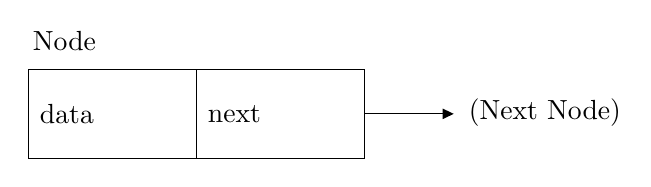
\begin{tikzpicture}[x=0.75pt,y=0.75pt,yscale=-1,xscale=1]
%uncomment if require: \path (0,300); %set diagram left start at 0, and has height of 300

%Straight Lines [id:da8067314459176902] 
\draw    (413,149.25) -- (453,149.25) ;
\draw [shift={(456,149.25)}, rotate = 180] [fill={rgb, 255:red, 0; green, 0; blue, 0 }  ][line width=0.08]  [draw opacity=0] (5.36,-2.57) -- (0,0) -- (5.36,2.57) -- cycle    ;

% Text Node
\draw    (251,127.75) -- (332,127.75) -- (332,170.75) -- (251,170.75) -- cycle  ;
\draw (291.5,149.25) node   [align=left] {\begin{minipage}[lt]{52.36pt}\setlength\topsep{0pt}
data
\end{minipage}};
% Text Node
\draw    (332,127.75) -- (413,127.75) -- (413,170.75) -- (332,170.75) -- cycle  ;
\draw (372.5,149.25) node   [align=left] {\begin{minipage}[lt]{52.36pt}\setlength\topsep{0pt}
next
\end{minipage}};
% Text Node
\draw (252,108) node [anchor=north west][inner sep=0.75pt]   [align=left] {Node};
% Text Node
\draw (462,140.75) node [anchor=north west][inner sep=0.75pt]   [align=left] {(Next Node)};


\end{tikzpicture}
\caption{链表的一个节点}
\label{fig: 链表的一个节点}
\end{figure}

如图 \ref{fig: 链表的一个节点} 所示, 链表中的一个元素成为一个\textbf{节点} (node),
一个节点内包含了该元素存储的数据, 和指向该元素的后继元的一个指针, 我们称之为
\lstinline|next| 指针.

\subsection{双向链表}

双向链表 (doubly linked list) 的基本思想是在每一个节点都增加一个指向其前一个节点的
指针. 它增加了空间的需求, 但是使得链表的删除操作得到简化.

\begin{figure}[H]
    \centering


\tikzset{every picture/.style={line width=0.75pt}} %set default line width to 0.75pt        

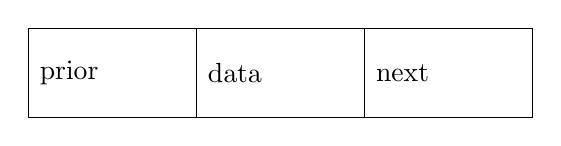
\begin{tikzpicture}[x=0.75pt,y=0.75pt,yscale=-1,xscale=1]
%uncomment if require: \path (0,300); %set diagram left start at 0, and has height of 300


% Text Node
\draw    (272,106.75) -- (353,106.75) -- (353,149.75) -- (272,149.75) -- cycle  ;
\draw (312.5,128.25) node   [align=left] {\begin{minipage}[lt]{52.36pt}\setlength\topsep{0pt}
data
\end{minipage}};
% Text Node
\draw    (191,106.75) -- (272,106.75) -- (272,149.75) -- (191,149.75) -- cycle  ;
\draw (231.5,128.25) node   [align=left] {\begin{minipage}[lt]{52.36pt}\setlength\topsep{0pt}
prior
\end{minipage}};
% Text Node
\draw    (353,106.75) -- (434,106.75) -- (434,149.75) -- (353,149.75) -- cycle  ;
\draw (393.5,128.25) node   [align=left] {\begin{minipage}[lt]{52.36pt}\setlength\topsep{0pt}
next
\end{minipage}};


\end{tikzpicture}
\caption{双向链表的节点}
\end{figure}

\begin{figure}[H]
    \centering


\tikzset{every picture/.style={line width=0.75pt}} %set default line width to 0.75pt        

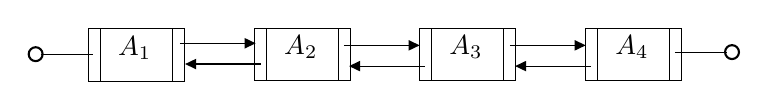
\begin{tikzpicture}[x=0.75pt,y=0.75pt,yscale=-1,xscale=1]
%uncomment if require: \path (0,300); %set diagram left start at 0, and has height of 300

%Flowchart: Prodefined Process [id:dp004630555102067779] 
\draw   (96.5,148) -- (142.5,148) -- (142.5,173.25) -- (96.5,173.25) -- cycle ; \draw   (102.25,148) -- (102.25,173.25) ; \draw   (136.75,148) -- (136.75,173.25) ;

%Straight Lines [id:da3813384726256295] 
\draw    (140.5,155) -- (174,155) ;
\draw [shift={(177,155)}, rotate = 180] [fill={rgb, 255:red, 0; green, 0; blue, 0 }  ][line width=0.08]  [draw opacity=0] (5.36,-2.57) -- (0,0) -- (5.36,2.57) -- cycle    ;
%Flowchart: Prodefined Process [id:dp5223096431915815] 
\draw   (176.5,147.75) -- (222.5,147.75) -- (222.5,173) -- (176.5,173) -- cycle ; \draw   (182.25,147.75) -- (182.25,173) ; \draw   (216.75,147.75) -- (216.75,173) ;

%Straight Lines [id:da6128812605175352] 
\draw    (146,165) -- (179.5,165) ;
\draw [shift={(143,165)}, rotate = 0] [fill={rgb, 255:red, 0; green, 0; blue, 0 }  ][line width=0.08]  [draw opacity=0] (5.36,-2.57) -- (0,0) -- (5.36,2.57) -- cycle    ;
%Straight Lines [id:da5013934657765772] 
\draw    (219.5,156) -- (253,156) ;
\draw [shift={(256,156)}, rotate = 180] [fill={rgb, 255:red, 0; green, 0; blue, 0 }  ][line width=0.08]  [draw opacity=0] (5.36,-2.57) -- (0,0) -- (5.36,2.57) -- cycle    ;
%Flowchart: Prodefined Process [id:dp7067864189341271] 
\draw   (256,147.75) -- (302,147.75) -- (302,173) -- (256,173) -- cycle ; \draw   (261.75,147.75) -- (261.75,173) ; \draw   (296.25,147.75) -- (296.25,173) ;

%Straight Lines [id:da13466336164029968] 
\draw    (225,166) -- (258.5,166) ;
\draw [shift={(222,166)}, rotate = 0] [fill={rgb, 255:red, 0; green, 0; blue, 0 }  ][line width=0.08]  [draw opacity=0] (5.36,-2.57) -- (0,0) -- (5.36,2.57) -- cycle    ;
%Straight Lines [id:da19760915206438967] 
\draw    (299.5,156) -- (333,156) ;
\draw [shift={(336,156)}, rotate = 180] [fill={rgb, 255:red, 0; green, 0; blue, 0 }  ][line width=0.08]  [draw opacity=0] (5.36,-2.57) -- (0,0) -- (5.36,2.57) -- cycle    ;
%Flowchart: Prodefined Process [id:dp38385435488735953] 
\draw   (336,147.75) -- (382,147.75) -- (382,173) -- (336,173) -- cycle ; \draw   (341.75,147.75) -- (341.75,173) ; \draw   (376.25,147.75) -- (376.25,173) ;

%Straight Lines [id:da4490195316506437] 
\draw    (305,166) -- (338.5,166) ;
\draw [shift={(302,166)}, rotate = 0] [fill={rgb, 255:red, 0; green, 0; blue, 0 }  ][line width=0.08]  [draw opacity=0] (5.36,-2.57) -- (0,0) -- (5.36,2.57) -- cycle    ;
%Straight Lines [id:da9113595039119798] 
\draw    (379,159.25) -- (404.15,159.25) ;
\draw [shift={(406.5,159.25)}, rotate = 0] [color={rgb, 255:red, 0; green, 0; blue, 0 }  ][line width=0.75]      (0, 0) circle [x radius= 3.35, y radius= 3.35]   ;
%Straight Lines [id:da3482654725085852] 
\draw    (73.35,160.25) -- (98.5,160.25) ;
\draw [shift={(71,160.25)}, rotate = 0] [color={rgb, 255:red, 0; green, 0; blue, 0 }  ][line width=0.75]      (0, 0) circle [x radius= 3.35, y radius= 3.35]   ;

% Text Node
\draw (109.5,150.4) node [anchor=north west][inner sep=0.75pt]    {$A_{1}$};
% Text Node
\draw (189.5,150.15) node [anchor=north west][inner sep=0.75pt]    {$A_{2}$};
% Text Node
\draw (269,150.15) node [anchor=north west][inner sep=0.75pt]    {$A_{3}$};
% Text Node
\draw (349,150.15) node [anchor=north west][inner sep=0.75pt]    {$A_{4}$};


\end{tikzpicture}
\caption{一个双向链表}
\end{figure}

\begin{figure}[H]
    \centering


\tikzset{every picture/.style={line width=0.75pt}} %set default line width to 0.75pt        

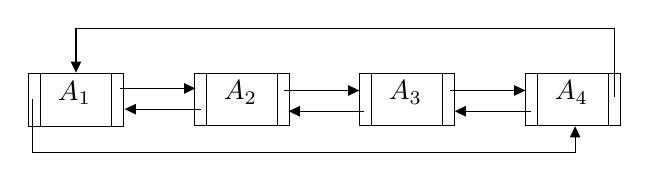
\begin{tikzpicture}[x=0.75pt,y=0.75pt,yscale=-1,xscale=1]
%uncomment if require: \path (0,300); %set diagram left start at 0, and has height of 300

%Flowchart: Prodefined Process [id:dp9104042449241202] 
\draw   (201.5,126) -- (247.5,126) -- (247.5,151.25) -- (201.5,151.25) -- cycle ; \draw   (207.25,126) -- (207.25,151.25) ; \draw   (241.75,126) -- (241.75,151.25) ;

%Straight Lines [id:da18290980624291586] 
\draw    (245.5,133) -- (279,133) ;
\draw [shift={(282,133)}, rotate = 180] [fill={rgb, 255:red, 0; green, 0; blue, 0 }  ][line width=0.08]  [draw opacity=0] (5.36,-2.57) -- (0,0) -- (5.36,2.57) -- cycle    ;
%Flowchart: Prodefined Process [id:dp6779023038048237] 
\draw   (281.5,125.75) -- (327.5,125.75) -- (327.5,151) -- (281.5,151) -- cycle ; \draw   (287.25,125.75) -- (287.25,151) ; \draw   (321.75,125.75) -- (321.75,151) ;

%Straight Lines [id:da05078733209108777] 
\draw    (251,143) -- (284.5,143) ;
\draw [shift={(248,143)}, rotate = 0] [fill={rgb, 255:red, 0; green, 0; blue, 0 }  ][line width=0.08]  [draw opacity=0] (5.36,-2.57) -- (0,0) -- (5.36,2.57) -- cycle    ;
%Straight Lines [id:da7779253189888817] 
\draw    (324.5,134) -- (358,134) ;
\draw [shift={(361,134)}, rotate = 180] [fill={rgb, 255:red, 0; green, 0; blue, 0 }  ][line width=0.08]  [draw opacity=0] (5.36,-2.57) -- (0,0) -- (5.36,2.57) -- cycle    ;
%Flowchart: Prodefined Process [id:dp4721319671372639] 
\draw   (361,125.75) -- (407,125.75) -- (407,151) -- (361,151) -- cycle ; \draw   (366.75,125.75) -- (366.75,151) ; \draw   (401.25,125.75) -- (401.25,151) ;

%Straight Lines [id:da8077639830606532] 
\draw    (330,144) -- (363.5,144) ;
\draw [shift={(327,144)}, rotate = 0] [fill={rgb, 255:red, 0; green, 0; blue, 0 }  ][line width=0.08]  [draw opacity=0] (5.36,-2.57) -- (0,0) -- (5.36,2.57) -- cycle    ;
%Straight Lines [id:da45511898958045416] 
\draw    (404.5,134) -- (438,134) ;
\draw [shift={(441,134)}, rotate = 180] [fill={rgb, 255:red, 0; green, 0; blue, 0 }  ][line width=0.08]  [draw opacity=0] (5.36,-2.57) -- (0,0) -- (5.36,2.57) -- cycle    ;
%Flowchart: Prodefined Process [id:dp0076852552006743124] 
\draw   (441,125.75) -- (487,125.75) -- (487,151) -- (441,151) -- cycle ; \draw   (446.75,125.75) -- (446.75,151) ; \draw   (481.25,125.75) -- (481.25,151) ;

%Straight Lines [id:da414081469968975] 
\draw    (410,144) -- (443.5,144) ;
\draw [shift={(407,144)}, rotate = 0] [fill={rgb, 255:red, 0; green, 0; blue, 0 }  ][line width=0.08]  [draw opacity=0] (5.36,-2.57) -- (0,0) -- (5.36,2.57) -- cycle    ;
%Straight Lines [id:da9830686882631294] 
\draw    (484,137.25) -- (484,104) -- (224.5,104) -- (224.5,122.4) ;
\draw [shift={(224.5,125.4)}, rotate = 270] [fill={rgb, 255:red, 0; green, 0; blue, 0 }  ][line width=0.08]  [draw opacity=0] (5.36,-2.57) -- (0,0) -- (5.36,2.57) -- cycle    ;
%Straight Lines [id:da28391834524539317] 
\draw    (465,154.25) -- (465,164) -- (203.5,164) -- (203.5,138.25) ;
\draw [shift={(465,151.25)}, rotate = 90] [fill={rgb, 255:red, 0; green, 0; blue, 0 }  ][line width=0.08]  [draw opacity=0] (5.36,-2.57) -- (0,0) -- (5.36,2.57) -- cycle    ;

% Text Node
\draw (454,128.15) node [anchor=north west][inner sep=0.75pt]    {$A_{4}$};
% Text Node
\draw (374,128.15) node [anchor=north west][inner sep=0.75pt]    {$A_{3}$};
% Text Node
\draw (294.5,128.15) node [anchor=north west][inner sep=0.75pt]    {$A_{2}$};
% Text Node
\draw (214.5,128.4) node [anchor=north west][inner sep=0.75pt]    {$A_{1}$};


\end{tikzpicture}
\caption{一个没有表头的双向循环链表}
\end{figure}

\begin{code}
    \lstset{
        moreemph={data, prior, next},
        emphstyle=\color{class_field},
    }
    \lstinputlisting[language=C]{/Users/strik0r/CLionProjects/DataStructure/DoublyLinkedList-ggh.c}
\end{code}

\begin{table}[H]
    \centering
    \caption{线性表链式存储方式的比较}
    \begin{tabular}{cccc}
        \hline
        & 找首元素节点 & 找表尾节点 & 找 $p$ 节点的前一个节点 \\ 
        \hline
    \end{tabular}
\end{table}

\section{线性表的应用}

\subsection{多项式 ADT}

\subsubsection{一元多项式的表示}

次数非负的多项式 $f(x) = \sum_{i=0}^n a_ix^i$, 其中 $a_n \ne 0$, 则可以用一个线性表 $Q$ 来表示, 其中
\[ Q = \left(a_0, a_1, a_2, \cdots, a_n \right), \]
假设 $h(x) = \sum_{i=0}^m b_ix^i$, 其中 $b_m \ne 0$ 且 $m<n$, 那么 $f(x) + h(x)$
可以用线性表表示为
\[ \left(a_0 + b_0, a_1 + b_1, \cdots, a_m+b_m, a_{m+1}, a_{m+2}, \cdots, a_n\right). \]

\subsubsection{一元多项式的存储}

如先前所述, 线性表的存储方式有顺序表和链表两种.

我们把零系数较多的多项式称为稀疏多项式. 显然, 如果对稀疏多项式采用顺序表存储, 那无疑会造成
存储空间的极大浪费, 例如, 多项式
$f(x) = 1 + 5x^{10000} + 7x^{20000}$
的顺序表存储需要 $200001$ 个空间, 但实际有效的存储数据只有 $3$ 个, 因此, 对于稀疏多项式来说
采用链式存储更能节省储存空间.

由于非零系数较多的非稀疏多项式可以用简单的数组实现, 讨论的价值不高, 本节主要讨论稀疏多项式的链式存储.
我们采用双向链表作为存储结构来实现多项式 ADT.

\subsubsection{多项式的节点结构}

在双向链表中, 节点 \lstinline|Node| 含有 \lstinline|prior|、\lstinline|data| 和
\lstinline|next| 三个数据域, 为了用一个节点存储多项式中的一项, 
我们需要把 \lstinline|data| 数据域明确为
多项式中某项的系数 \lstinline|coef| 和某项的次数 \lstinline|exp|.
多项式的节点结构如图 \ref{一元多项式的节点结构} 所示.

\begin{figure}[H]
    \centering
    % 图的内容


    \tikzset{every picture/.style={line width=0.75pt}} %set default line width to 0.75pt        

    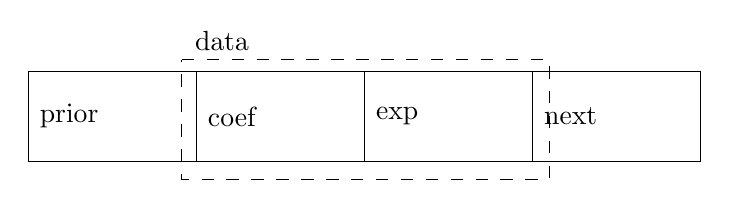
\begin{tikzpicture}[x=0.75pt,y=0.75pt,yscale=-1,xscale=1]
    %uncomment if require: \path (0,300); %set diagram left start at 0, and has height of 300
    
    %Shape: Rectangle [id:dp43237688915398287] 
    \draw  [dash pattern={on 4.5pt off 4.5pt}] (204,121) -- (381,121) -- (381,178.5) -- (204,178.5) -- cycle ;
    
    % Text Node
    \draw    (292,126.75) -- (373,126.75) -- (373,169.75) -- (292,169.75) -- cycle  ;
    \draw (332.5,148.25) node   [align=left] {\begin{minipage}[lt]{52.36pt}\setlength\topsep{0pt}
    exp
    \end{minipage}};
    % Text Node
    \draw    (130,126.75) -- (211,126.75) -- (211,169.75) -- (130,169.75) -- cycle  ;
    \draw (170.5,148.25) node   [align=left] {\begin{minipage}[lt]{52.36pt}\setlength\topsep{0pt}
    prior
    \end{minipage}};
    % Text Node
    \draw    (373,126.75) -- (454,126.75) -- (454,169.75) -- (373,169.75) -- cycle  ;
    \draw (413.5,148.25) node   [align=left] {\begin{minipage}[lt]{52.36pt}\setlength\topsep{0pt}
    next
    \end{minipage}};
    % Text Node
    \draw    (211,126.75) -- (292,126.75) -- (292,169.75) -- (211,169.75) -- cycle  ;
    \draw (251.5,148.25) node   [align=left] {\begin{minipage}[lt]{52.36pt}\setlength\topsep{0pt}
    coef
    \end{minipage}};
    % Text Node
    \draw (207,105.75) node [anchor=north west][inner sep=0.75pt]   [align=left] {\begin{minipage}[lt]{22.58pt}\setlength\topsep{0pt}
    \begin{center}
    data
    \end{center}
    
    \end{minipage}};
    
    
    \end{tikzpicture}
    % \includegraphics*[width=\textwidth]{imagefile}

    \caption{一元多项式的节点结构}
    \label{一元多项式的节点结构}
\end{figure}

节点结构的声明如下:
\begin{lstlisting}[language=C]
struct DNode {
    double coef;
    int exp;
    struct DNode *prior, *next;
};
typedef struct DNode *DNode;
// DNode 是一个指向 DNode 结构的指针, 在后续代码中一般用于指向节点
\end{lstlisting}

\subsubsection{应用: 高精度计算圆周率}

\[ \dfrac{\pi}{2} = \sum_{k=0}^\infty \dfrac{(2k)!!}{(2k+1)!!}\left(
    \dfrac{1}{2}
\right)^k. \]

\section{栈 ADT}

\subsection{栈的定义}

\textbf{栈} (stack) 是一种{\kaishu 限制插入和删除只能在一个位置上进行}的表,
该位置是表的末端, 称为\textbf{栈顶} (stack top), 相对的, 表的第一个元素称为\textbf{栈底} 
(stack bottom). 对栈的基本操作主要有两种:
\begin{itemize}[itemsep=0pt]
    \item \lstinline|push()|: 进栈操作, 相当于插入元素.
    \item \lstinline|pop()|: 出栈操作, 相当于取出元素, 它返回位于栈顶的元素.
\end{itemize}
由于在栈中只有位于栈顶的元素才是可访问的, 因此后进入的元素一定先被取出, 于是又称为
\textbf{后进先出表} (Last In, First Out, LIST).

\begin{figure}[H]
    \centering
    % 图的内容


    \tikzset{every picture/.style={line width=0.75pt}} %set default line width to 0.75pt        

    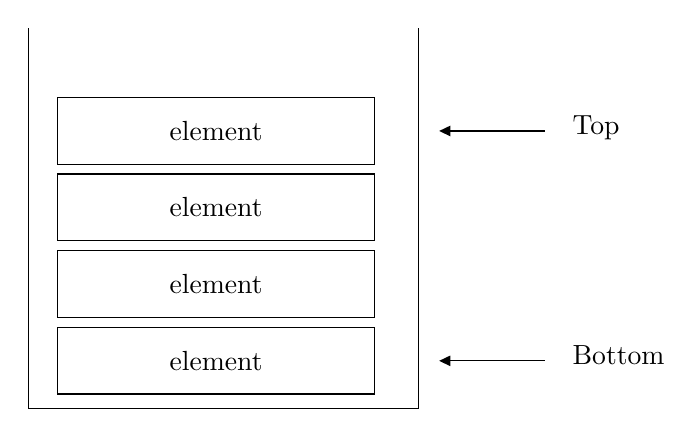
\begin{tikzpicture}[x=0.75pt,y=0.75pt,yscale=-1,xscale=1]
    %uncomment if require: \path (0,300); %set diagram left start at 0, and has height of 300
    
    %Straight Lines [id:da9240706265381634] 
    \draw    (54,73.5) -- (54,256.5) -- (242,256.5) -- (242,73.5) ;
    %Straight Lines [id:da8868586304966674] 
    \draw    (255,123) -- (303,123) ;
    \draw [shift={(252,123)}, rotate = 0] [fill={rgb, 255:red, 0; green, 0; blue, 0 }  ][line width=0.08]  [draw opacity=0] (5.36,-2.57) -- (0,0) -- (5.36,2.57) -- cycle    ;
    %Straight Lines [id:da6463485015431351] 
    \draw    (255,233.75) -- (303,233.75) ;
    \draw [shift={(252,233.75)}, rotate = 0] [fill={rgb, 255:red, 0; green, 0; blue, 0 }  ][line width=0.08]  [draw opacity=0] (5.36,-2.57) -- (0,0) -- (5.36,2.57) -- cycle    ;
    
    % Text Node
    \draw    (68,217.75) -- (221,217.75) -- (221,249.75) -- (68,249.75) -- cycle  ;
    \draw (144.5,233.75) node   [align=left] {\begin{minipage}[lt]{101.32pt}\setlength\topsep{0pt}
    \begin{center}
    element
    \end{center}
    
    \end{minipage}};
    % Text Node
    \draw    (68,180.75) -- (221,180.75) -- (221,212.75) -- (68,212.75) -- cycle  ;
    \draw (144.5,196.75) node   [align=left] {\begin{minipage}[lt]{101.32pt}\setlength\topsep{0pt}
    \begin{center}
    element
    \end{center}
    
    \end{minipage}};
    % Text Node
    \draw    (68,143.75) -- (221,143.75) -- (221,175.75) -- (68,175.75) -- cycle  ;
    \draw (144.5,159.75) node   [align=left] {\begin{minipage}[lt]{101.32pt}\setlength\topsep{0pt}
    \begin{center}
    element
    \end{center}
    
    \end{minipage}};
    % Text Node
    \draw    (68,107) -- (221,107) -- (221,139) -- (68,139) -- cycle  ;
    \draw (144.5,123) node   [align=left] {\begin{minipage}[lt]{101.32pt}\setlength\topsep{0pt}
    \begin{center}
    element
    \end{center}
    
    \end{minipage}};
    % Text Node
    \draw (315,114.5) node [anchor=north west][inner sep=0.75pt]   [align=left] {Top};
    % Text Node
    \draw (315,225.25) node [anchor=north west][inner sep=0.75pt]   [align=left] {Bottom};
    
    
    \end{tikzpicture}
    % \includegraphics*[width=\textwidth]{imagefile}

    \caption{栈}
    \label{栈}
\end{figure}

由于栈的限制存取的特性, 入栈操作、出栈操作的时间和空间复杂度都是 $O(1)$.
当某个数据集合只涉及在一端插入和删除数据, 并且满足后进先出、先进后出的特性的时候,
我们就应该首选栈作为数据结构.

\begin{example}
    若进栈序列为 $1,2,3,4$, 允许边进边出, 但每次出栈都要记录出栈的元素, 则不可能得到的出栈序列是?
    \begin{tasks}[label={\Alph*.}](2)
        \task $3,2,1,4$
        \task $3,2,4,1$
        \task $4,2,3,1$
        \task $2,3,4,1$
    \end{tasks}
    \begin{cmt}
        要注意栈的后进先出原则, 如果第一个出栈元素是 $4$, 那么说明在此之前四个数已经全部进栈了,
        $4$ 出栈后的栈顶应该是 $3$. 于是本题选择 C 选项. 关于这一类题型有一个技巧, 那就是
        优先分析那些{\kaishu 靠后入栈的元素最先出栈}的序列——越往后入栈的元素越提前出来, 只能说明这前面的元素
        都已经入栈了, 并且此前并没有发生过出栈操作.
    \end{cmt}
\end{example}

\begin{example}
    假设有五个整数以 $1,2,3,4,5$ 的顺序入栈, 允许边进边出, 每次出栈记录出栈元素, 出栈序列
    为 $3,5,4,2,1$, 那么栈大小至少为?
    \begin{tasks}[label={\Alph*.}](4)
        \task 2
        \task 3
        \task 4
        \task 5
    \end{tasks}
    \begin{cmt}
        能够满足题目要求的最小栈大小等于该过程中栈中元素的最大个数. 我们不妨分析一下,
        首先入栈: \[ (1,2,3), \]
        观察到出栈序列的第一个数是 $3$, 于是此时发生出栈操作,
        \[ (1,2), \]
        入栈, \[ (1,2,4,5), \]
        依次出栈直到栈空, 出栈序列恰为 $3,5,4,2,1$, 因此该过程是符合题目要求的操作过程.
        考虑到出栈不可能增加栈中元素的个数,
        因此该过程中栈内最多只有 $4$ 个元素, 因此本题选 C.
    \end{cmt}
\end{example}

\subsection{栈的实现方式}

数组和链表是基础的数据结构, 许多数据结构的实现都依赖于数组和链表. 栈 ADT 可以使用数组和链表
来实现, 使用数组实现的栈称为顺序栈, 使用链表实现的称为链式栈.

用数组实现的顺序栈见程序清单 \ref{code: arrayStack}. 我们首先定义了用于实现
顺序栈的 \lstinline|ArrayStack| 类, 然后声明了若干标识栈的状态的变量: 首先是存放栈中元素的数组
\lstinline|items|, 其次是栈顶的下标 \lstinline|top|,
以及栈的大小 \lstinline|capacity|.

由于这段 Java 代码并不设计任何高级语法, 并且注释相对详细, 因此我们就不在正文中专门解释了.

\begin{code}
    \label{code: arrayStack}
    \lstinline|ArrayStack.java|
    \lstset{moreemph={items, top, capacity},
    emphstyle=\color{class_field}}
    \lstinputlisting[language=Java,
    ]{/Users/strik0r/Documents/IdeaProjects/Hello/src/cn/edu/nwpu/software/strik0r/data_structures/linear_structure/stack/ArrayStack.java}
\end{code}

\appendix
% 设置 chapter 标题样式
\titleformat{\chapter}[hang]{\centering\heiti\Large\bfseries}{附录\,\thechapter}{1em}{}
\renewcommand{\chaptermark}[1]{\markboth{附录 \thechapter\, #1}{}}

\onecolumn
\begin{thebibliography}{1}
    \addcontentsline{toc}{chapter}{参考文献}
    \bibitem{Mark}
    [美] Mark Allen Weiss. 数据结构与算法分析—— C 语言描述 (原书第 2 版)
    (典藏版) / Data Structures and Algorithm Analysis in C,
    Second Edition [M]. 冯舜玺译. 北京: 机械工业出版社, 2019.
    \bibitem{Michael}
    [美] Michael Goodrich, [美] Roberto Tamassia, 
    [美] Michael H. Goldwasser. 数据结构与算法: Python 语言实现
    / Data Structures and Algorithms in Python [M].
    张晓等译. 北京: 机械工业出版社, 2018.
    \bibitem{Cormen}
    [美] Thomas H. Cormen, [美] Charles E. Leiserson,
    [美] Ronald L. Rivest, [美] Clifford Stein.
    算法导论 (原书第 3 版) / Introduction to Algorithms, Third Edition [M].
    殷建平等译. 北京: 机械工业出版社, 2013.
    \bibitem{耿国华}
    耿国华等. 数据结构: 用 C 语言描述 (第 2 版) [M].
    北京: 高等教育出版社, 2015.
    \bibitem{王道数据结构}
    王道论坛组. 2024 年数据结构考研复习指导 [M]. 北京: 电子工业出版社, 2022.
    \bibitem{严蔚敏}
    严蔚敏, 李冬梅, 吴伟民. 数据结构: C 语言版: 双色版: 第 2 版 [M].
    北京: 人民邮电出版社, 2022.
    \bibitem{习题解析与实验指导}
    李冬梅, 田紫微. 数据结构习题解析与实验指导: 第 2 版 [M]. 北京: 人民邮电出版社, 2022.
\end{thebibliography}

\newpage
\thispagestyle{empty}
\vspace*{5cm}
\begin{center}
    \includegraphics*[width=\textwidth]{pic/i_love_npu.jpeg}
    \large
    公诚勇毅 \quad 永矢毋忘

    中华灿烂 \quad 工大无疆
\end{center}
\vspace*{13em}
\begin{center}
    \small
    本文档由\textbf{钱锋}编写, 钱锋保留一切权利.

    文档中出现的部分素材来源于网络, 笔者承诺这些素材仅供学习交流之用, 
    它们的原作者保留一切权利.

    2023 年 \quad 西北工业大学 \quad 中国西安 
\end{center}

\end{document}